\documentclass[11pt,a4paper,margin=0.5in]{report}

\usepackage[utf8]{inputenc}
\usepackage[francais]{babel}
\usepackage[margin=1in,footskip=0.25in]{geometry}
\usepackage{graphicx}
\usepackage[document]{ragged2e}
\usepackage{hyperref}

\title{ 
\includegraphics[scale=0.33]{m3.png} \\[0.25in]Modular Mind Mapping - M3 \\ UPMC M2 STL TPDEV Projet}
\author{Elias Boutaleb}
\date{\today}

\begin{document}

\maketitle
\tableofcontents

\chapter{Introduction}

\begin{center}
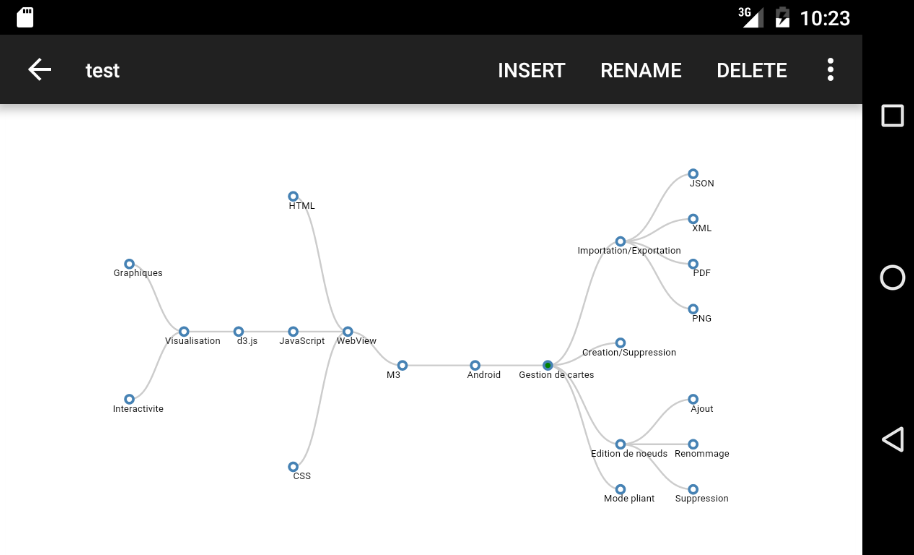
\includegraphics[scale=0.5]{mm.png} \\[0.25in]
\end{center}

\section{Contexte}

Modular Mind Mapping (M3) est un logiciel de cartographie conceptuelle (mindmapping) qui permet d'organiser des informations de manière
visuelle sous forme d'arborescence utilisant le framework de visualisation de données d3.js\footnote{\url{http://d3js.org/}}.

On part d'un thème donné, puis on y associe différentes idées, des images, d'autres mots, des hyperliens.

\clearpage

Il existe déjà plusieurs applications de ce type sur le Google Play Store mais plusieures choses ne convenaient
pas au développeur de M3:
soit elles ne sont pas gratuites, par exemple avec xxx, dont la version complète coûte \\

\begin{center}
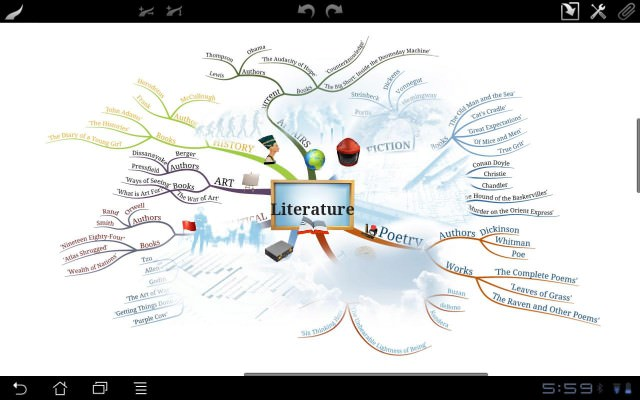
\includegraphics[scale=0.33]{ex1.jpg} \\[0.25in]
\end{center}

soit elles sont limitées dans les options offertes quant à l'importation et exportation des cartes. \\

\begin{center}
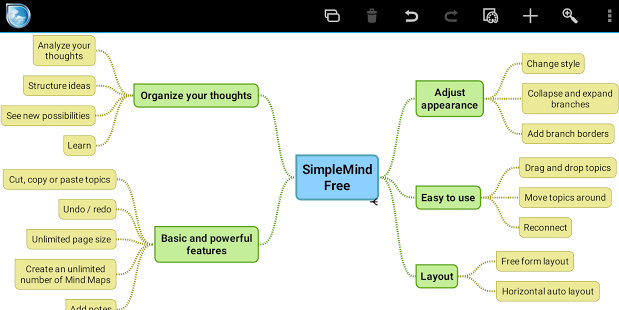
\includegraphics[scale=0.33]{unnamed.png} \\[0.25in]
\end{center}

De surcroît, j'ai jugé qu'il pourrait être intéressant de pouvoir intégrer les capacités de visualisation de données de d3.js à une mindmap, d'ailleurs cela n'a pas encore été fait à ma connaissance.

\section{Fonctionnalités}

Un utilisateur a pour possibilité sur le site de :

Il supportera l'exportation de cartes en SVG, PNG, PDF, JSON.
Il supportera l'importation de cartes en JSON et FreeMind XML (.mm).
Les cartes pourront être chargées ou enregistrées sur l'appareil.
Création et suppression de cartes
Une manipulation interactive de la carte sera possible (ajout/suppression/déplacement des noeuds, changement du layout de l'arbre)
Import de données qui seront visualisées
L'insertion d'images est envisagée.
Changement du fond, des couleurs
Inline webview de graphs d3
%\begin{itemize}
%\end{itemize}

\chapter{Manuel utilisateur}

\section{Description de l'interface}

\begin{center}
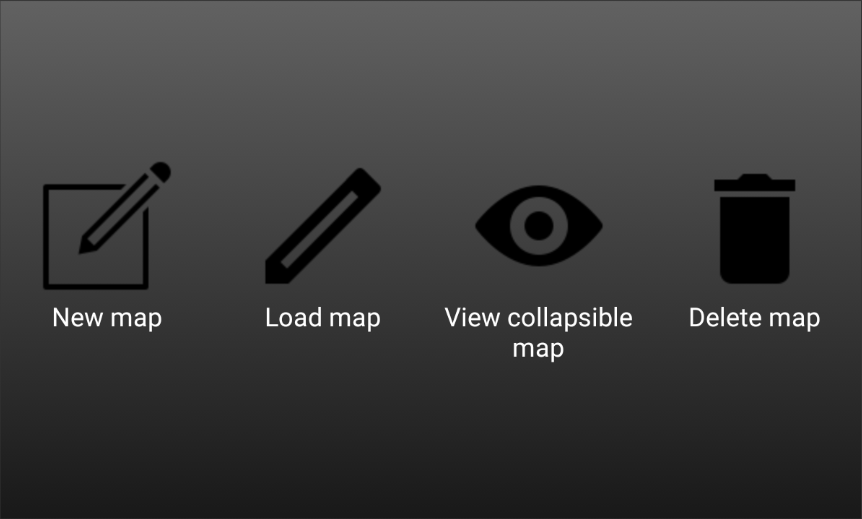
\includegraphics[scale=0.33]{dashb.png} \\[0.25in]
\end{center}

\begin{center}
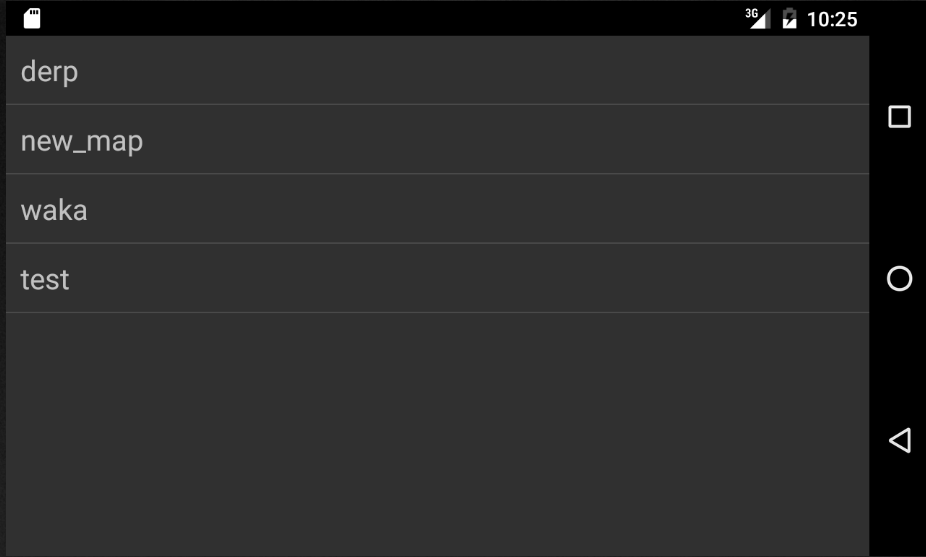
\includegraphics[scale=0.33]{choice.png} \\[0.25in]
\end{center}

\begin{center}
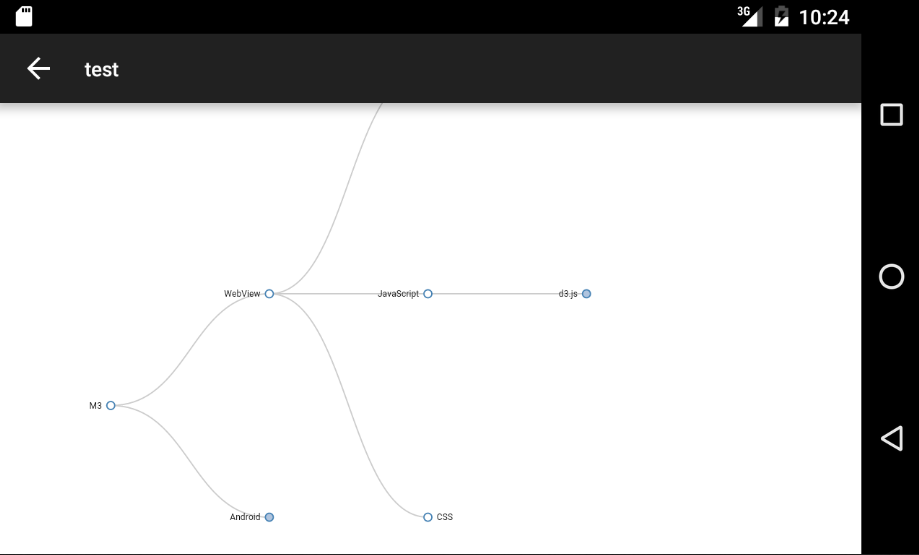
\includegraphics[scale=0.33]{coll.png} \\[0.25in]
\end{center}

\clearpage

\chapter{Architecture de l'application}

\section{Choix techniques}

\vspace{0.5cm}

module TimeEntry.\\[0.1in]
La manipulation des cartes se fait avec l'aide de l'API Google Maps.

\chapter{Extensions et améliorations}

\section{Avantages de l'application}
\begin{enumerate}
    \item Elle est extensible, grâce à l'architecture MVC qui rend facile l'ajout de nouvelles pages et des routes URL correspondantes.
    %\begin{itemize}
    %\end{itemize}
    \item Elle via l'API REST.
\end{enumerate}

\section{Inconvénients de l'application}

\section{Améliorations à faire}

\section{Extensions possibles}
Les fonctionnalités suivantes pourraient être ajoutées à l'application:

\end{document}
